\documentclass{decar-wsd}    % Document style

\usepackage{decar-common}    % Commonly used commands and packages
\usepackage{decar-dynamics}  % Dynamics commands (load only if needed)
\usepackage{decar-lie}       % Lie group commands (load only if needed)
% \usepackage{todonotes}        % Load whatever other packages you want here
\usepackage{decar-post}      % Packages that must be loaded last

\title{UWB Calibration}
\author{Mohammed Shalaby}

\begin{document}

\maketitle

\section{Alternative Double-Sided Two-Way Ranging}

\subsection{Standard Single-Sided Two-Way Ranging}

\begin{figure}
    \centering
    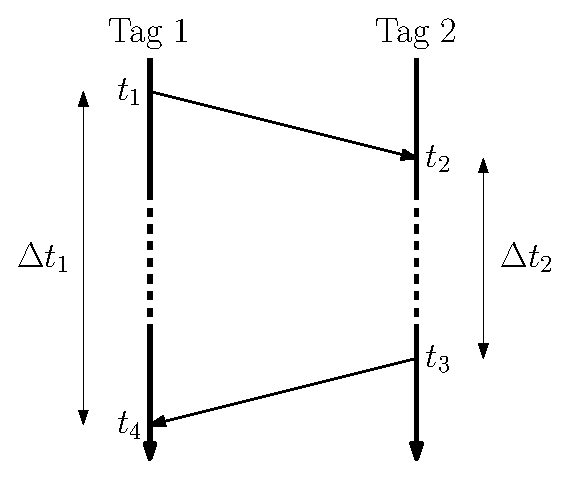
\includegraphics[width=5cm]{figs/standard_twr.eps}
    \caption{Single-sided TWR.}
    \label{fig:ss_twr}
\end{figure}

Standard two-way ranging (TWR) is shown in Fig. \ref{fig:ss_twr}, where
\begin{align}
    \Delta t_1 &= t_4 - t_1, \\
    \Delta t_2 &= t_3 - t_2,
\end{align}
The time-of-flight of a signal between two tags is
\begin{align}
    t_f = \f{1}{2} \left( \Delta t_1 - \Delta t_2 \right).
\end{align}
However, the clock rates of each tag is different than the true global reference time, and the measured signal is then modelled as
\begin{align}
    \hat{t}_f &= \f{1}{2} \left( \left(1 + \gamma_1 \right) \Delta t_1 - \left( 1 + \gamma_2 \right) \Delta t_2 \right).
\end{align}
This then results in an error of
\begin{align}
    \hat{t}_f - t_f &= \f{1}{2} \left( \left(1 + \gamma_1 \right) \Delta t_1 - \left( 1 + \gamma_2 \right) \Delta t_2 \right) -  \f{1}{2} \left( \Delta t_1 - \Delta t_2 \right) \\
    &= \f{1}{2} \gamma_1 \Delta t_1 - \f{1}{2} \gamma_2 \Delta t_2 \\
    &= \f{1}{2} \gamma_1 (2 t_f + \Delta t_2) - \f{1}{2} \gamma_2 \Delta t_2 \\
    &= \gamma_1 t_f + \f{1}{2} \left( \gamma_1 - \gamma_2 \right) \Delta t_2.
\end{align}
Given that typically $t_2 >> t_f$, it is the main source of error. In fact, typically, $t_2$ is in the order of hundreds of microseconds or a few milliseconds, and this can result in significant bias in the range measurements.

\subsection{Reversed Double-Sided Two-Way Ranging}

\begin{figure}
    \centering
    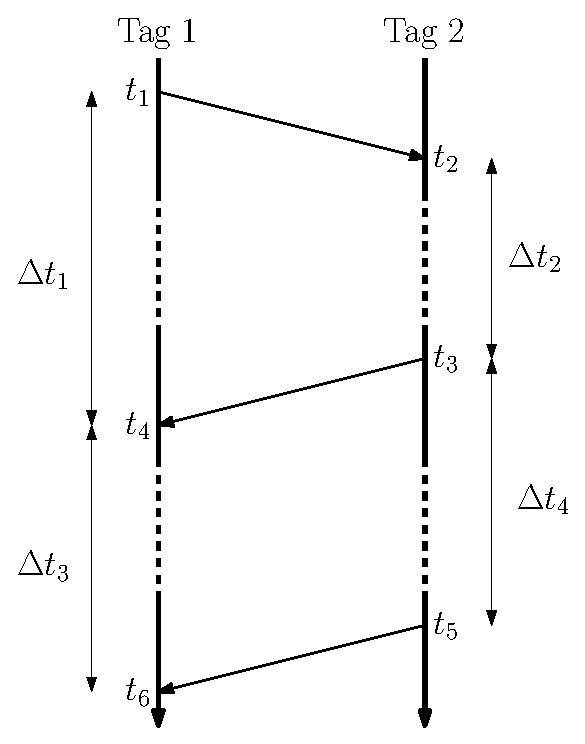
\includegraphics[width=5cm]{figs/multiplicative_twr.eps}
    \caption{Reversed Double-sided TWR.}
    \label{fig:rev_ds_twr}
\end{figure}

An alternative TWR algorithm involves sending an additional signal in what is referred to as double-sided TWR. The term "reversed" here refers to the fact that in the subsequent implementation, the last message's direction is referred as compared to typical double-sided TWR as shown in Fig. \ref{fig:rev_ds_twr}, where
\begin{align}
    \Delta t_1 &= t_4 - t_1, \\
    \Delta t_2 &= t_3 - t_2, \\
    \Delta t_3 &= t_6 - t_4, \\
    \Delta t_4 &= t_5 - t_3,
\end{align}
From Fig. \ref{fig:rev_ds_twr}, it can be seen that if the clock rates of the two tags are exactly the same, then $\Delta t_3 = \Delta t_4$. This information can then be used to convert $\Delta t_2$ from the clock of Tag 2 to the clock of Tag 1 when performing TWR, as given by
\begin{align}
    t_f = \f{1}{2} \left( \Delta t_1 - \f{\Delta t_3}{\Delta t_4} \Delta t_2 \right).
\end{align}
The recorded measurement is then
\begin{align}
    \hat{t}_f &= \f{1}{2} \left( \left(1 + \gamma_1 \right) \Delta t_1 - \f{\left(1 + \gamma_1 \right) \Delta t_3}{\left(1 + \gamma_2 \right) \Delta t_4} \left( 1 + \gamma_2 \right) \Delta t_2 \right) \\
    &= \f{1}{2} \left( \left(1 + \gamma_1 \right) \Delta t_1 - \left(1 + \gamma_1 \right) \f{\Delta t_3}{\Delta t_4} \Delta t_2 \right),
\end{align}
and the error in the measurement is given by
\begin{align}
    \hat{t}_f - t_f &= \f{1}{2} \left( \left(1 + \gamma_1 \right) \Delta t_1 - \left(1 + \gamma_1 \right) \f{\Delta t_3}{\Delta t_4} \Delta t_2 \right) - \f{1}{2} \left( \Delta t_1 - \f{\Delta t_3}{\Delta t_4} \Delta t_2 \right) \\
    &= \f{1}{2} \gamma_1 \left( \Delta t_1 - \f{\Delta t_3}{\Delta t_4} \Delta t_2 \right) \\
    &= \f{1}{2} \gamma_1 t_f.
\end{align}
This is significantly better than standard two-way ranging, as the time-of-flight is typically in the order of nanoseconds.

\section{Antenna Delay Calibration}

On the UWB modules, the Decawave chip performs the timestamping, while the antenna performs the actual communication. The time between a chip timestamps the time of transmission and the antenna actually transmits the signal is referred to as the antenna transmission delay $d^t$, while the time between an antenna receives a signal and the time the chip timestamps the time of transmission is referred to as the antenna reception delay $d^r$. Looking back at Figure \ref{fig:rev_ds_twr}, the actual measured time-stamps are therefore
\begin{align}
    \hat{t}_1 &= t_1 + d_1^t, \\
    \hat{t}_2 &= t_2 - d_2^r, \\
    \hat{t}_3 &= t_3 + d_2^t, \\
    \hat{t}_4 &= t_4 - d_1^r, \\ 
    \hat{t}_5 &= t_5 + d_2^t, \\
    \hat{t}_6 &= t_6 - d_1^r,
\end{align}
where $d_i^t$ and $d_i^r$ are the antenna transmission and reception delays of Tag $i$, respectively.

The calibration procedure described by DW is specific to standard TWR, and does not suggest any optimization but rather a heuristic approach to calibrate the delays. In what follows, a linear least-squares approach is proposed for the reversed double-sided TWR algorithm.

The true time-of-flight of a signal as a function of the measured time-stamps can be modelled as
\begin{align}
    \Delta \hat{t}_1 &= \Delta t_1 - d_1^r - d_1^t, \\
    \Delta \hat{t}_2 &= \Delta t_2 + d_2^t + d_2^r, \\
    \Delta \hat{t}_3 &= \Delta t_3, \\
    \Delta \hat{t}_4 &= \Delta t_4,
\end{align}
The actual measured deltas as a function of the true deltas and the antenna delays are given by
\begin{align}
    t_f &= \f{1}{2} \left( \Delta {t}_1 - \f{ \Delta {t}_3}{\Delta {t}_4} \Delta {t}_2 \right) \\
    &= \f{1}{2} \left( \Delta \hat{t}_1 + \underbrace{ d_1^r + d_1^t}_{d_1} - \f{ \Delta \hat{t}_3}{\Delta \hat{t}_4} \left( \Delta t_2  \underbrace{ - d_2^t - d_2^r}_{-d_2} \right) \right)
\end{align}
Clearly, transmission and reception delays can be combined into one delay variable to be optimized for every tag. For one measurement, this can be re-written as
\begin{align}
    \bma{cc} \f{1}{2} & \f{1}{2}K \ema \bma{c} d_1 \\ d_2 \ema &= \bma{c} t_f - \f{1}{2} \Delta \hat{t}_1 + \f{1}{2} K \Delta \hat{t}_2 \ema \\
    &\triangleq b,
\end{align}
where 
\begin{equation}
    K \triangleq \f{ \Delta \hat{t}_3}{\Delta \hat{t}_4}.
\end{equation}
Stacking many measurements between two tags yields
\begin{align}
    \bma{cc} \f{1}{2} & \f{1}{2}K^1 \\ \vdots & \vdots \\ \f{1}{2} & \f{1}{2}K^n \ema \bma{c} d_1 \\ d_2 \ema &= \bma{c} b^1 \\ \vdots \\ b^n \ema.
\end{align}
This however is unobservable, as the left-hand side matrix is not full column rank. As suggested by Decawave, the calibration procedure should involve at least 3 tags, thus yielding the following linear least-squares problem:
\begin{align}
    \bma{ccc} \f{1}{2} & \f{1}{2}K^1_{12} &  \\ \vdots & \vdots &  \\ \f{1}{2} & \f{1}{2}K^1_{12} & \\ \\ \hline \\ \f{1}{2} & & \f{1}{2}K^1_{13} \\ \vdots &  & \vdots \\ \f{1}{2} & & \f{1}{2}K^n_{13} \\ \\ \hline \\ & \f{1}{2} & \f{1}{2}K^1_{23} \\ & \vdots & \vdots \\ & \f{1}{2} & \f{1}{2}K^n_{23} \ema \bma{c} d_1 \\ d_2 \\ d_3 \ema &= \bma{c} b_{12}^1 \\ \vdots \\ b_{12}^n \\ \\ \hline \\ b_{13}^1 \\ \vdots \\ b_{13}^n \\ \\ \hline \\ b_{23}^1 \\ \vdots \\ b_{23}^n \ema.
\end{align}

\subsection{Results}



\section{Variance of Measurements}

\subsection{Single-Sided (SS) TWR}

The SS TWR protocol calculates the time-of-flight measurement as
\begin{align}
    t_f &= \f{1}{2}\left( \Delta t_1 - \Delta t_2 \right) \\
    &= \f{1}{2} \left( t_4 - t_1 - t_3 + t_2 \right).
\end{align}
Given that both tags have potentially skewed clocks, and accommodating for randomness, the time-of-flight measurement is modelled as
\begin{align}
    \hat{t}_f = \f{1}{2} \left( \left( 1 + \gamma_1\right) \left( t_4 - t_1 + \eta_4 - \eta_1 \right) - \left( 1 + \gamma_2\right) \left( t_3 - t_2 + \eta_3 - \eta_2 \right) \right).
\end{align}

The time-of-flight measurement error is then
\begin{equation}
    e \triangleq \hat{t}_f - t_f = \f{1}{2} \left( \gamma_1 \left( t_4 - t_1 \right) + \left( 1 + \gamma_1\right) \left( \eta_4 - \eta_1 \right) - \gamma_2 \left( t_3 - t_2 \right) - \left( 1 + \gamma_2\right) \left( \eta_3 - \eta_2 \right) \right),
\end{equation}
where $\eta_i \sim \mathcal{N} \left(0, R\right)$, and $\eta_i$, $\eta_j$ are mutually independent for all $i,j \in \{1,2,3,4\}, i \neq j$.

The expected value of the error is then
\begin{align}
    \mathbb{E} [e] &= \f{1}{2} \left( \gamma_1 \left( t_4 - t_1 \right) - \gamma_2 \left( t_3 - t_2 \right) \right) \\
    &= \f{1}{2} \left( \gamma_1 \left( 2t_f + t_3 - t_2 \right) - \gamma_2 \left( t_3 - t_2 \right) \right) \\
    &= \gamma_1 t_f + \f{1}{2} \left(\gamma_1 - \gamma_2\right) \left( t_3 - t_2 \right),
\end{align}
while the variance of the error is given by
\begin{align}
    \mathbb{E} \left[ (e - \mathbb{E}[e])(\cdot)^\trans \right] &= \mathbb{E} \left[ \left(\f{1}{2} \left( 1 + \gamma_1\right) \left( \eta_4 - \eta_1 \right) - \f{1}{2}\left( 1 + \gamma_2\right) \left( \eta_3 - \eta_2 \right) \right) (\cdot)^\trans \right]^\trans \\
    &= \f{1}{4}\left( 1+\gamma_1 \right)\left( R_4 + R_1 \right) + \f{1}{4} \left(1 + \gamma_2 \right) \left( R_3 + R_2 \right) \\
    &= \f{1}{2}\left( 1+\gamma_1 \right) R + \f{1}{2} \left(1 + \gamma_2 \right) R \\
    &= R + \f{1}{2}(\gamma_1 + \gamma_2) R.
\end{align}

\subsection{Reversed Double-Sided (DS) TWR}

The DS TWR protocol involves calculating the time-of-flight measurement as 
\begin{align}
    t_f &= \f{1}{2} \left( \Delta t_1 - \f{\Delta t_3}{\Delta t_4} \Delta t_2 \right) \\
    &= \f{\Delta t_1 \Delta t_4 - \Delta t_3 \Delta t_2}{2 \Delta t_4} \\
    &= \f{(t_4 - t_1)(t_5 - t_3) - (t_6 - t_4)(t_3 - t_2)}{2(t_5 - t_3)}.
\end{align}
In the presence of noise and clock skew, the time-of-flight measurement is modelled as 
\begin{align}
    \hat{t}_f &= \f{(1+\gamma_1)(1+\gamma_2)(t_4 - t_1 + \eta_4 - \eta_1)(t_5 - t_3 + \eta_5 - \eta_3) - (1+\gamma_1)(1+\gamma_2)(t_6 - t_4 + \eta_6 - \eta_4)(t_3 - t_2 + \eta_3 - \eta_2)}{2(1+\gamma_2)(t_5 - t_3 + \eta_5 - \eta_3)} \\
    &= \f{(1+\gamma_1)(t_4 - t_1 + \eta_4 - \eta_1)(t_5 - t_3 + \eta_5 - \eta_3) - (1+\gamma_1)(t_6 - t_4 + \eta_6 - \eta_4)(t_3 - t_2 + \eta_3 - \eta_2)}{2(t_5 - t_3 + \eta_5 - \eta_3)} \\
    &= (1+\gamma_1) \f{(t_4 - t_1 + \eta_4 - \eta_1)(t_5 - t_3 + \eta_5 - \eta_3) - (t_6 - t_4 + \eta_6 - \eta_4)(t_3 - t_2 + \eta_3 - \eta_2)}{2(t_5 - t_3 + \eta_5 - \eta_3)}.
\end{align}
The error in the time-of-flight measurement is then
\begin{align}
    e \triangleq \hat{t}_f - t_f &= \hspace{150pt} \ldots \\
    &= \hspace{155pt} \vdots \\
    &\approx \f{1}{2} \gamma_1 t_f + \f{1}{2} (1 + \gamma_1) \left[ \f{t_3 - t_2}{t_5 - t_3} \left( \eta_5 - \eta_3 + \eta_6 - \eta_4 \right) + \eta_4 - \eta_1 + \eta_2 - \eta_3 \right].
\end{align}
Therefore, the expected value for the error is
\begin{equation}
    \mathbb{E}[e] = \f{1}{2} \gamma_1 t_f,
\end{equation}
while the variance is 
\begin{align}
    \mathbb{E}[(e - \mathbb{E}[e])(\cdot)^\trans] &= \f{1}{4} (1 + \gamma_1)^2 \left[ \left(\f{t_3 - t_2}{t_5 - t_3}\right)^2 \left( R_5 - R_3 + R_6 - R_4 \right) + 2\left(\f{t_3 - t_2}{t_5 - t_3}\right) \left( R_3 + R_4 \right) + R_4 - R_1 + R_2 - R_3 \right] \\
    &= (1 + \gamma_1)^2 R + (1 + \gamma_1)^2 \left(\f{t_3 - t_2}{t_5 - t_3}\right) R + (1 + \gamma_1)^2 \left(\f{t_3 - t_2}{t_5 - t_3}\right)^2 R. \label{eq:ds_uncertainty}
\end{align}

Note that if $\gamma_1 = \gamma_2 = 0$, and as $t_5 - t_3 \rightarrow \infty$, the variance of DS TWR approaches that of the SS TWR. Given that this is not possible, $t_3 - t_2$ should be minimized while $t_5 - t_3$ should be maximized. The latter comes at a cost of measurement frequency, and therefore the user can design this value based on the application.

\subsubsection{Optimal Delay in DS TWR}

The amount of \emph{information} perceived in one unit of time is a function of two variables, 
\begin{enumerate}
    \item the uncertainty of the individual measurement, and
    \item the number of measurements in that unit of time. 
\end{enumerate}
As per \eqref{eq:ds_uncertainty}, the uncertainty in the individual measurement decreases as the delay in the second response (i.e., $\Delta t_4$, hereinafter referred to as \emph{the delay}) increases. However, as the delay increases, measurements occur less frequently, hence reducing the amount of information conveyed in a unit of time. As a result, the \emph{optimal} delay is one that is long enough to reduce the uncertainty of the individual measurement but short enough to ensure measurements are recorded at a sufficient frequency. 

Rewriting \eqref{eq:ds_uncertainty} in the absence of clock skews yields
\beq
    R_i \triangleq R + \f{\Delta t_2}{\Delta t_4} R + \left(\f{\Delta t_2}{\Delta t_4}\right)^2 R,
\eeq
for the individual measurement, where the time-stamps are replaced with the time delays for conciseness. The time-length of one measurement can be defined to be $T + \Delta t_4$ seconds long, where the time taken for all other signals and computational processing is lumped into the $T$ term as $\Delta t_4$ is the only variable of concern. Therefore, in one second, a total of $\f{1}{T + \Delta t_4}$ measurements occur, meaning that the overall uncertainty (inverse of information) of the measurements is given as
\begin{align}
    R_t &\triangleq (T + \Delta t_4) R_i \\
    %
    &= (T + \Delta t_4) R + \f{\Delta t_2 (T + \Delta t_4)}{\Delta t_4} R + \f{(\Delta t_2)^2(T + \Delta t_4)}{(\Delta t_4)^2} R \\
    %
    &= (T + \Delta t_4) R + \Delta t_2 T (\Delta t_4)^{-1} R + \Delta t_2 R + (\Delta t_2)^2 T (\Delta t_4)^{-2} R + (\Delta t_2)^2(\Delta t_4)^{-1} R. \label{eq:total_unc}
\end{align}
%
The derivative of \eqref{eq:total_unc} w.r.t. $\Delta t_4$ is then
\beq
    \f{\partial R_t}{\partial \Delta t_4} = R - \Delta t_2 T (\Delta t_4)^{-2} R - 2(\Delta t_2)^2 T (\Delta t_4)^{-3} R - (\Delta t_2)^2 (\Delta t_4)^{-2} R,
\eeq
and equating to 0 yields
\begin{align}
    0 &= (\Delta t_4)^3 - \Delta t_2 T \Delta t_4 - 2(\Delta t_2)^2 T - (\Delta t_2)^2 \Delta t_4 \\
    &= (\Delta t_4)^3 - \Delta t_2 (T + \Delta t_2) \Delta t_4 - 2(\Delta t_2)^2 T. \label{eq:optimal_delay}
\end{align}

The value for $T$ and $\Delta t_2$ can be determined experimentally and are application dependent. For the case where $T=6$ ms and $\Delta t_2=0.3$ ms, the optimal delay can be found analytically to be approximately 1.6 ms using \eqref{eq:optimal_delay}. This is also shown in Figure \ref{fig:optimal_delay}.

\begin{figure}[h!]
    \centering
    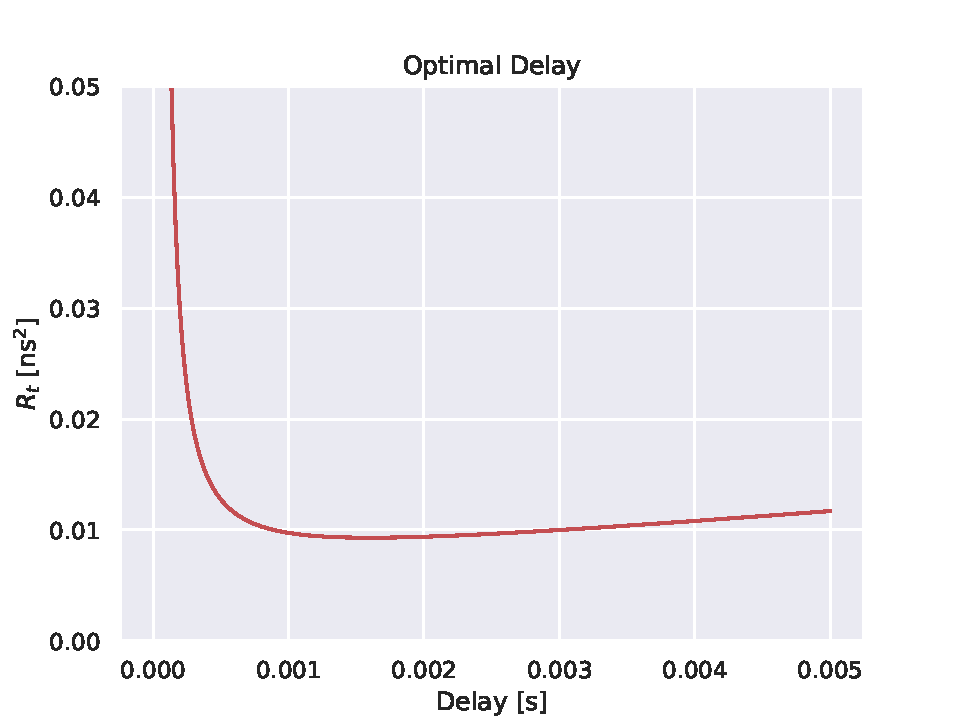
\includegraphics[width=0.6\textwidth]{figs/optimal_delay.pdf}
    \caption{Overall uncertainty as a function of second-response delay.}
    \label{fig:optimal_delay}
\end{figure}

\clearpage
\subsection{Examples}

\subsubsection{Older Examples}

\begin{figure}[h]
    \centering
    \begin{subfigure}[t]{0.5\textwidth}
        \centering
        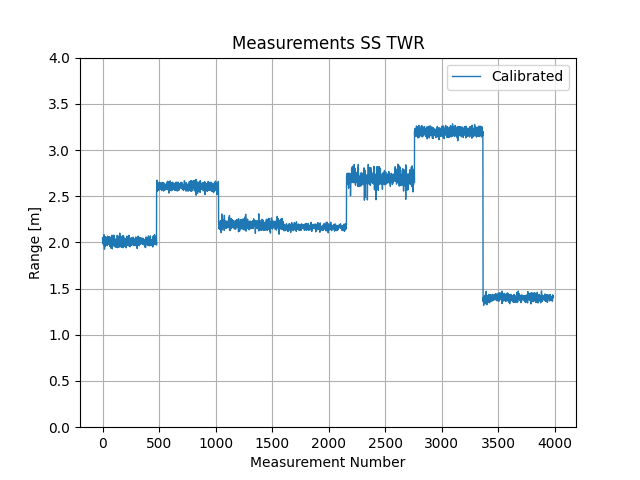
\includegraphics[width=\columnwidth]{figs/ss_twr.png}
        \caption{SS TWR.}
    \end{subfigure}%
    ~ 
    \begin{subfigure}[t]{0.5\textwidth}
        \centering
        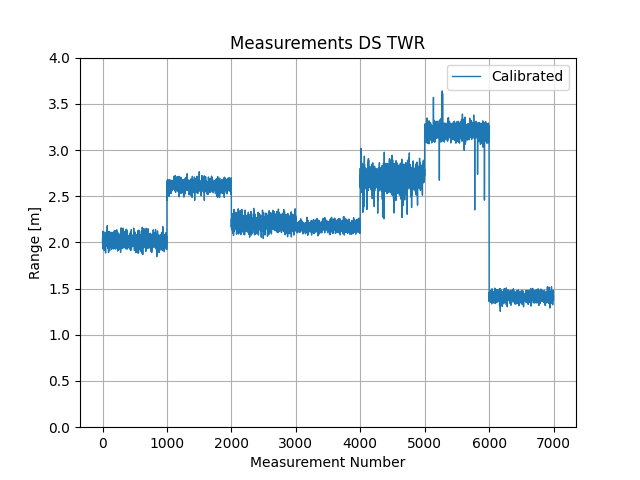
\includegraphics[width=\columnwidth]{figs/ds_twr.png}
        \caption{DS TWR.}
    \end{subfigure}
    \begin{subfigure}[t]{0.5\textwidth}
        \centering
        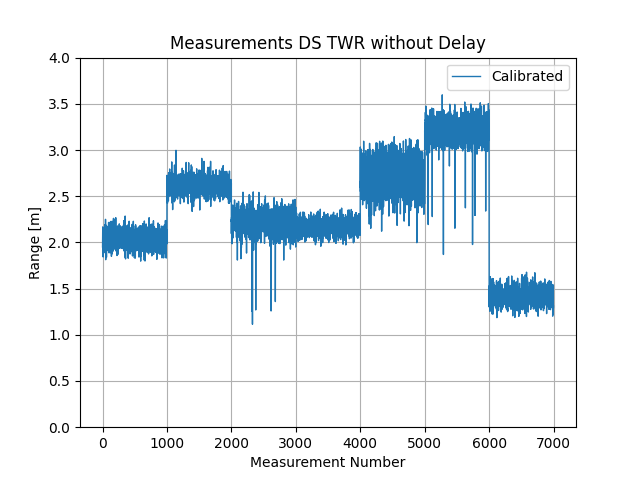
\includegraphics[width=\columnwidth]{figs/ds_twr_no_delay.png}
        \caption{DS TWR without pre-programmed delay between the transmission of signal 2 and signal 3.}
    \end{subfigure}
    \caption{The range measurements in 7 different formations. Note that the variance is dependent on both the ranging protocol and the relative pose.}
    \label{fig:range_7formations}
\end{figure}

\clearpage
\subsubsection{New Examples with fixed distance}

\begin{figure}[h]
    \centering
    \begin{subfigure}[t]{\textwidth}
        \centering
        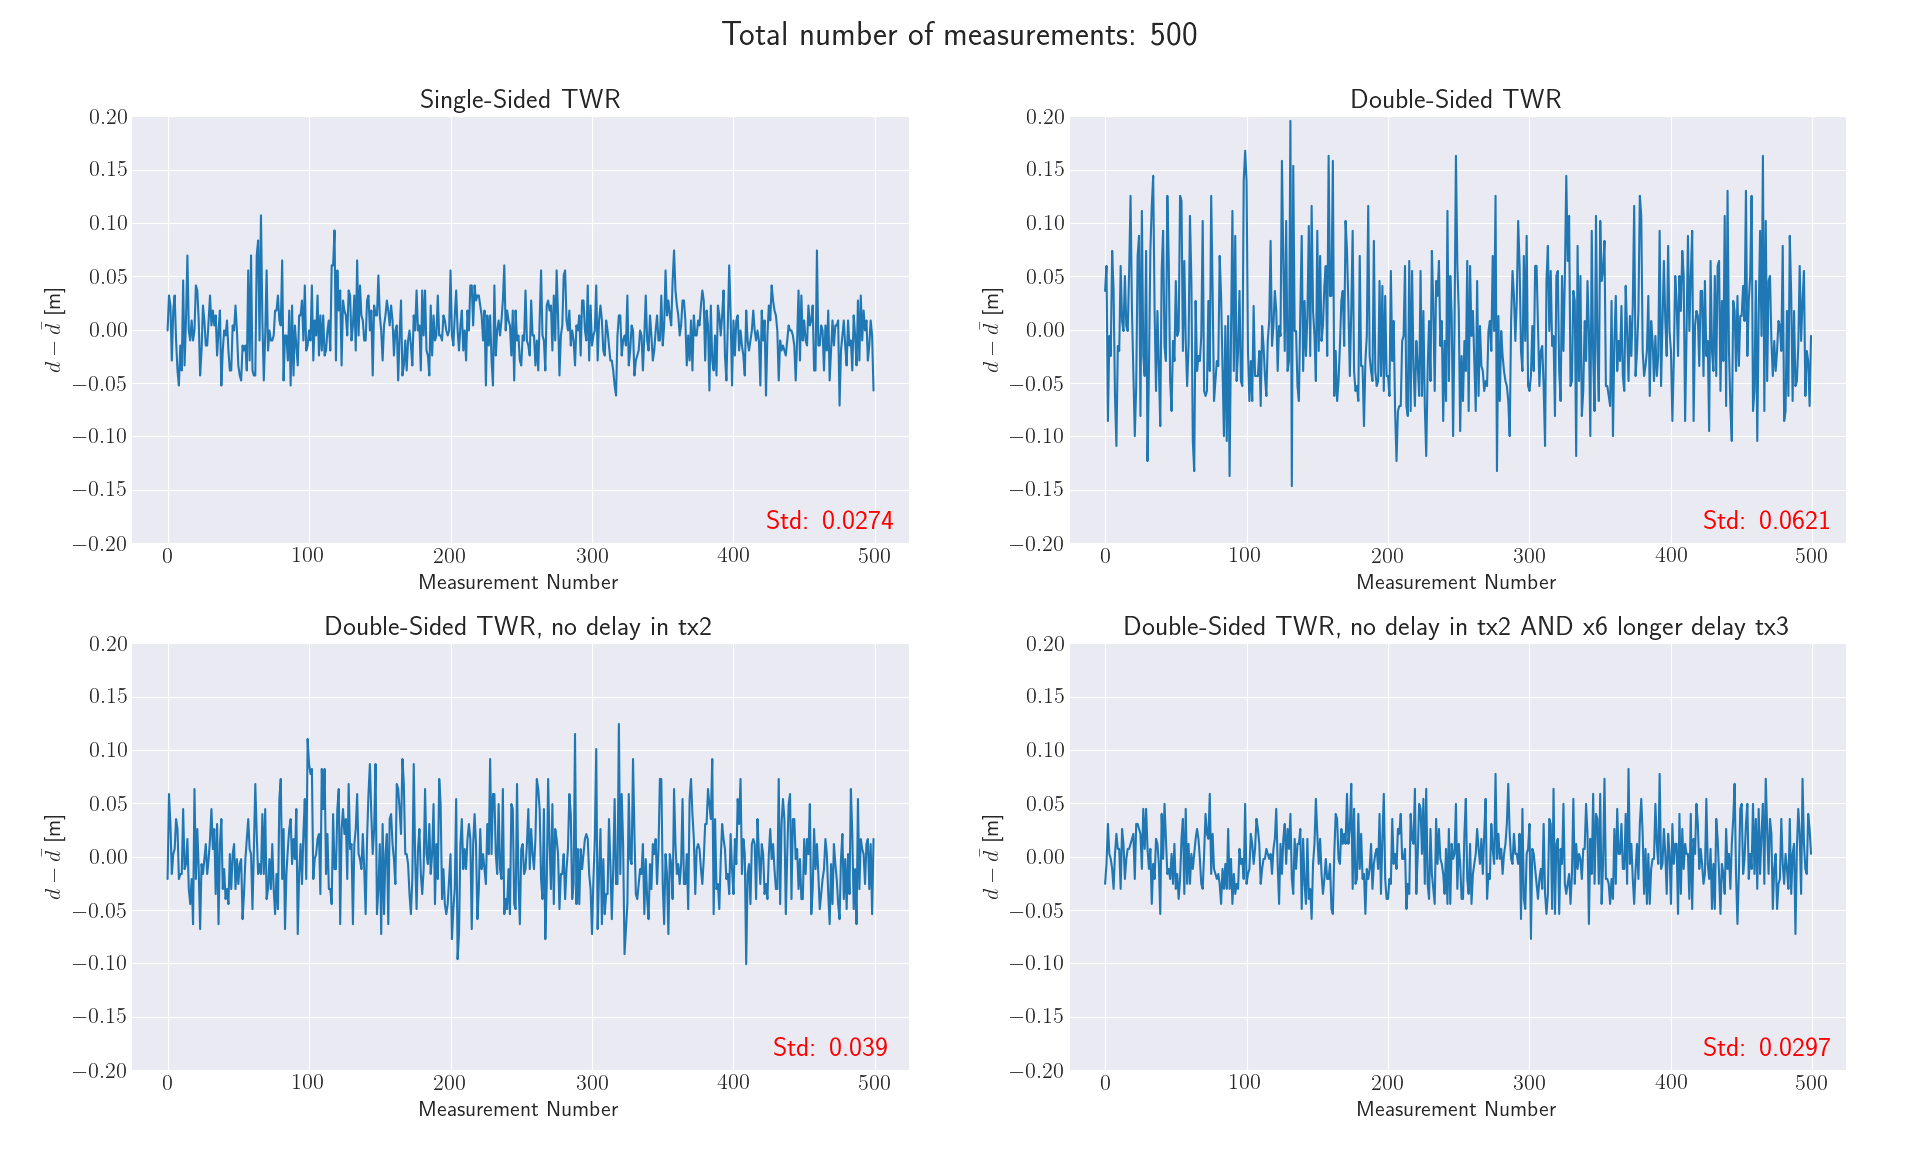
\includegraphics[width=0.8\columnwidth]{figs/std_comparison_500.png}
    \end{subfigure} \\
    \begin{subfigure}[t]{\textwidth}
        \centering
        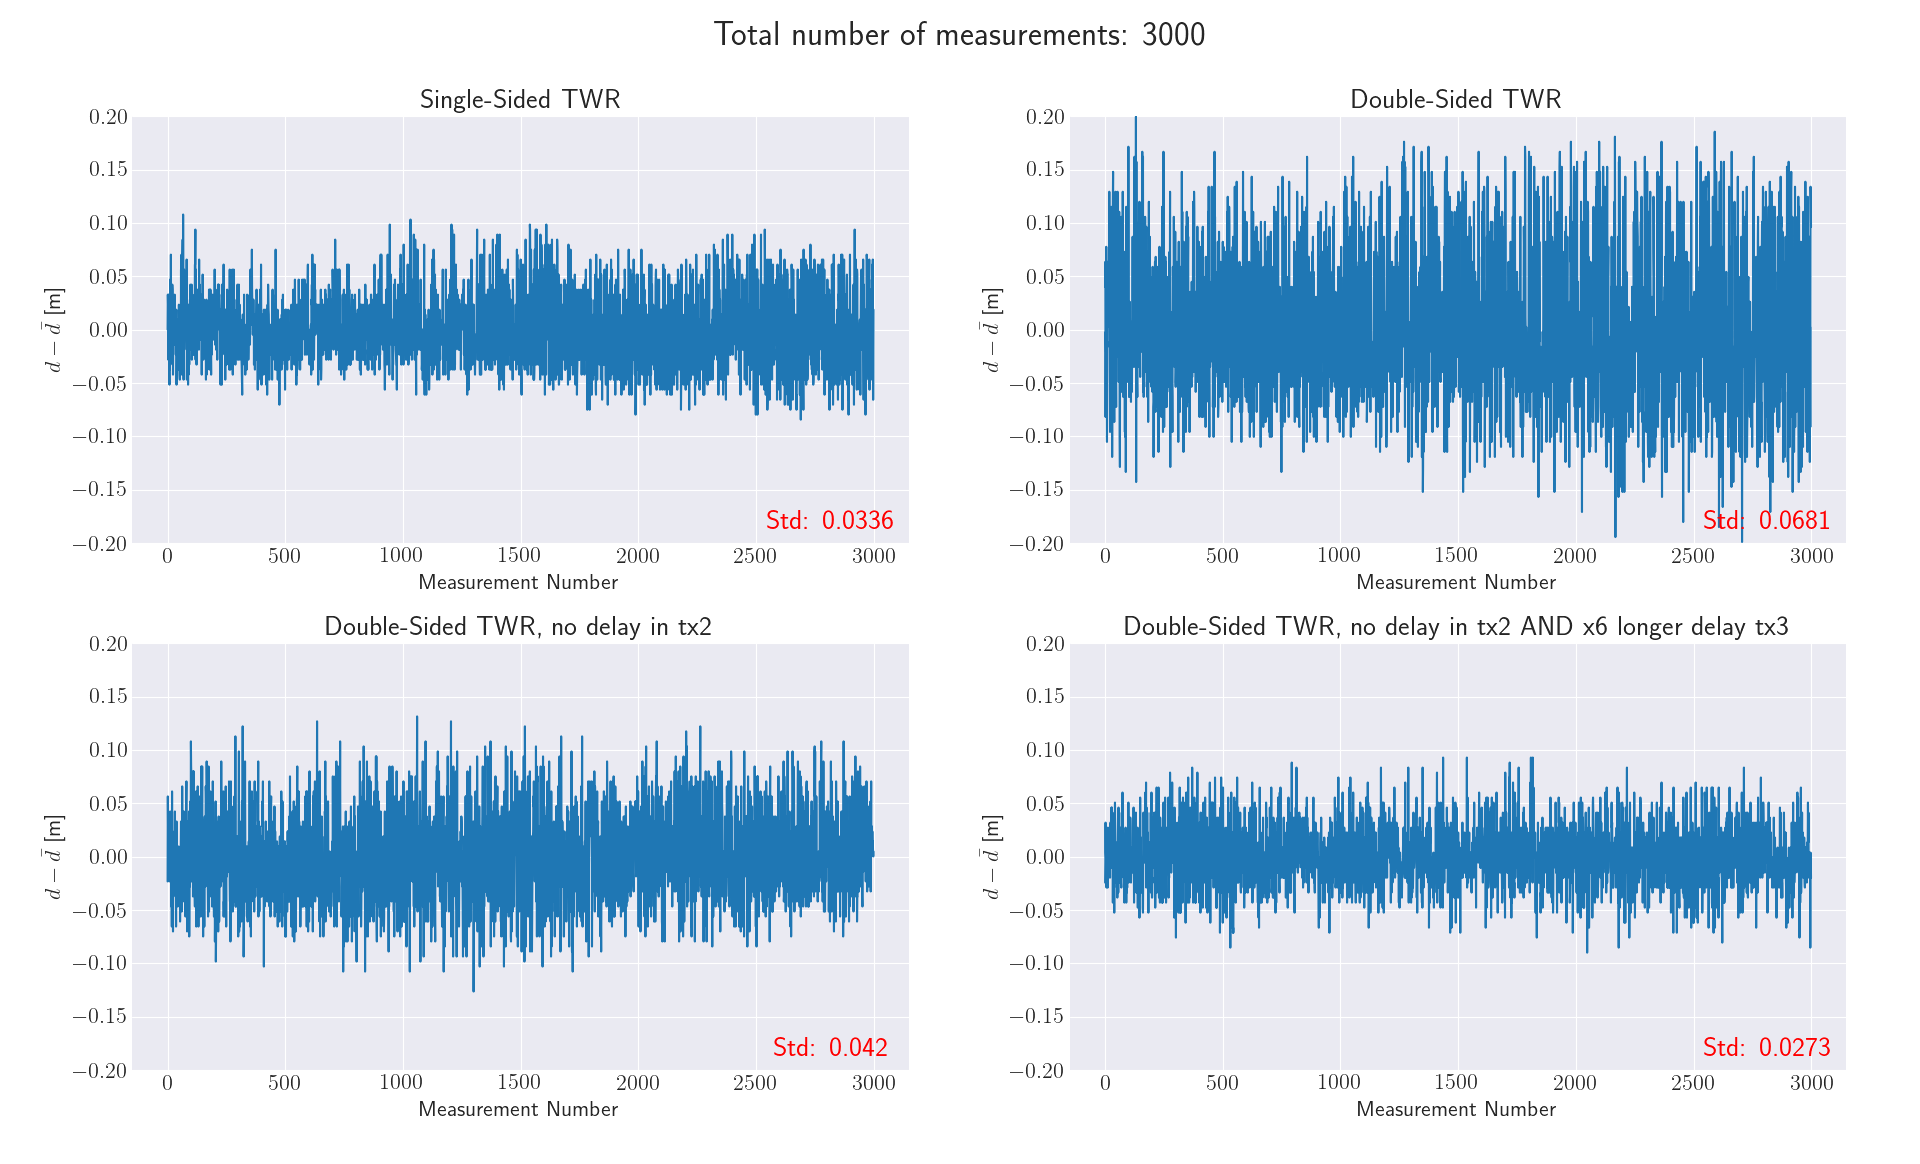
\includegraphics[width=0.8\columnwidth]{figs/std_comparison_3000.png}
    \end{subfigure}
    \caption{The variance of the range measurements, shown by plotting the difference between the range measurements and their mean. The variance for the single-sided TWR increases as the total number of measurements increases due to clock drift introducing time-varying bias even at a constant relative pose.}
    \label{fig:range_variance}
\end{figure}

\clearpage
\section{Power-correlated bias in double-sided TWR}

\begin{figure}
    \centering
    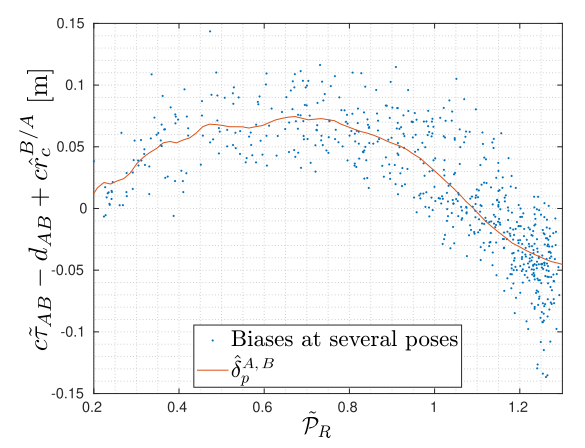
\includegraphics[width=0.7\textwidth]{figs/justins_data.png}
    \caption{Retrieved from \cite{Cano2022}. The bias vs. power values, using the assumption that $P_i^r = P_j^r$.}
    \label{fig:cano_bias}
\end{figure}

In \cite{Cano2022}, it is shown that the pose-dependent bias is actually correlated with the received signal power $P^r$ through a function $\rho(P^r)$. In the paper, the focus is on single-sided TWR, but the results for double-sided TWR are similar. In the absence of white noise and clock skew, the time-of-flight measurements can be modelled as a function of the true time-of-flight $t_f$, the power-correlated bias $\rho(P^r)$, and the transmission and reception delay, denoted $k^t$ and $k^r$ respectively. For tags $i$ and $j$, this yields the measurement model
\beq
    \label{eq:dstwr_model_powerAndDelay}
    y = t_f + \f{1}{2} \left( \rho(P^r_i) + \rho(P^r_j) \right) + \f{1}{2} \left( k_i^r - k_i^t \right) + \f{1}{2} \left( k_j^r - k_j^t \right),
\eeq
where the received power are the ones associated with the first two signals in a DS-TWR transaction. The antenna delay variables are addressed in the next section, but in \cite{Cano2022}, it is assumed that $P_i^r = P_j^r$ to collect the data shown in Figure \ref{fig:cano_bias}, which is not necessarily true. Therefore, this essentially means that in \cite{Cano2022}, the model is trained over values of $\f{1}{2} \left( \rho(P^r_i) + \rho(P^r_j) \right)$, which is not sufficient for one-way ranging examples, where the measurement model is given as
\beq
    y^{\text{owr}} = t_f + \delta_{ji} + \rho(P^r_j) + k^r_j - k^r_i.
\eeq
To overcome this assumption and for better calibration results, the learning procedure can be extended to 3 tags, $i,j,k$, where bias data is collected for 
\begin{align}
    \label{eq:owr_model_powerAndDelay}
    &\f{1}{2} \left( \rho(P^r_i) + \rho(P^r_j) \right), \\
    &\f{1}{2} \left( \rho(P^r_i) + \rho(P^r_k) \right), \\
    &\f{1}{2} \left( \rho(P^r_j) + \rho(P^r_k) \right).
\end{align}
This therefore allows the extraction of bias values corresponding to $\rho(P^r_i)$, $\rho(P^r_j)$, $\rho(P^r_k)$, individually.

\subsection{Using Gaussian Processes}

In \cite{Cano2022}, the emphasis of the calibration procedure is to correct the pose-dependent bias. However, as shown in Figure \ref{fig:range_7formations} and roughly in \ref{fig:cano_bias}, the variance of the measurements is also pose-dependent. Characterizing the uncertainty of the measurements is equally as important as correcting the bias in probabilistic frameworks.

Rather than using polynomials to fit the bias vs. power curve as is done in \cite{Cano2022} and Figure \ref{fig:cano_bias}, it could be possible to use Gaussian processes to fit a model to the curve, and thus obtain both a measure of bias and the uncertainty of the measurement based on the received power.

\clearpage
\section{Antenna delay calibration for Kalman filtering}

In \cite{Cano2022}, the antenna delay for every pair of tags is calibrated as one constant $K$. In essence, this $K$ incorporates the difference between the transmission and reception antenna delay for each tag involved in the TWR transaction, \ie, as shown by \eqref{eq:dstwr_model_powerAndDelay},
\beq
    K = \f{1}{2} \left( k_i^r - k_i^t \right) + \f{1}{2} \left( k_j^r - k_j^t \right).
\eeq
Nonetheless, this proposed calibration approach requires that the procedure is done for every pair of robots, which is tedious and not scalable. A simpler approach would be to utilize the fact that the antenna delay for each tag is constant. 

For $n$ tags to be calibrated, there are $2n$ unknown antenna delays and $n(n-1)$ measurements. When only TWR is to be utilized in the experiments, it is sufficient to calibrate only for the difference between the transmission and reception delay for every tag rather than the individual delays, thus halving the number of unknowns to $n$. This is due to the fact that the antenna delays only show as differences between the transmission and reception delays for each tag in TWR scenarios, as shown in \eqref{eq:dstwr_model_powerAndDelay}. Therefore, 3 tags are sufficient for the calibration procedure. When a new fourth tag is to be calibrated, there is only need for 2 tags in order to calibrate the one unknown.

Nonetheless, when other custom ranging protocols are utilized, such as one-way ranging as shown in \eqref{eq:owr_model_powerAndDelay}, it might be necessary to calibrate the individual antenna delays. Given there are $2n$ unknown delays and $n(n-1)$ measurements, at least 5 tags are required when none are pre-calibrated, and 3 tags are required to calibrate 1 new tag (2 calibrated, 1 to be calibrated). This is summarized in Table

\begin{table}[h!]
    \begin{center}
      \caption{The minimum number of tags required to deem antenna delay calibration observable.}
      \label{tab:delays}
      \begin{tabular}{p{0.18\linewidth}|p{0.18\linewidth}|p{0.28\linewidth}|p{0.3\linewidth}}
        \textbf{Ranging protocol} & \textbf{Delays calibrated} & \textbf{Number of uncalibrated tags required to calibrate all} & \textbf{Number of pre-calibrated tags required to calibrate 1 new tag}\\
        \hline
        TWR & $k^t - k^r$ & 3 & 1\\
        TWR \& OWR & $k^t$, $k^r$ & 5 & 2\\
      \end{tabular}
    \end{center}
  \end{table}



\clearpage
\section{Kalman Filtering}

Is this necessary? Need to calibrate antennae RX and TX delays separately?

\section{NLOS and Outlier Detection}

talk about convex hulls and detecting NLOS using mocap

show the outlier histograms and explain why almost inseparable

\clearpage

\addcontentsline{toc}{section}{References}
\bibliographystyle{ieeetr}
% \bibliographystyle{aiaa}
% \bibliographystyle{apacite}
% \bibliographystyle{plain} 
\bibliography{ref}
\end{document}
